\documentclass[
	12pt,
	openright,
	oneside,
	a4paper,
	english,
	french,
	spanish,
	brazil,	
	]{abntex2}

% ---
% PACOTES
% ---
\usepackage[T1]{fontenc}
\usepackage{pinhac}
% ---
% Pacotes fundamentais 
% ---
\usepackage{lmodern}			% Usa a fonte Latin Modern
\usepackage[T1]{fontenc}		% Selecao de codigos de fonte.
\usepackage[utf8]{inputenc}		% Codificacao do documento (conversão automática dos acentos)
\usepackage{indentfirst}		% Indenta o primeiro parágrafo de cada seção.
\usepackage{color}			% Controle das cores
\usepackage{graphicx}			% Inclusão de gráficos
\usepackage{microtype} 			% para melhorias de justificação
\usepackage{svg}
\usepackage{tikz}
\usepackage{xcolor}
\usepackage{wrapfig}

% ---
% Pacotes adicionais, usados apenas no âmbito do Modelo Canônico do abnteX2
% ---
\usepackage{lipsum}				% para geração de dummy text
% ---

% ---
% Pacotes de citações
% ---
\usepackage[brazilian,hyperpageref]{backref}	 % Paginas com as citações na bibl
\usepackage[alf]{abntex2cite}	% Citações padrão ABNT

\usepackage{fontspec}
\usepackage[T1]{fontenc}
\usepackage{amsfonts}
%\setmainfont{Liberation Sans}
% --- 
% CONFIGURAÇÕES DE PACOTES
% --- 
\usepackage{microtype} % Slightly tweak font spacing for aesthetics
\usepackage[utf8]{inputenc} % Required for including letters with accents
\usepackage[T1]{fontenc} % Use 8-bit encoding that has 256 glyphs
% ---
% Configurações do pacote backref
% Usado sem a opção hyperpageref de backref
\renewcommand{\backrefpagesname}{Citado na(s) página(s):~}
% Texto padrão antes do número das páginas
\renewcommand{\backref}{}
% Define os textos da citação
\renewcommand*{\backrefalt}[4]{
	\ifcase #1 %
		Nenhuma citação no texto.%
	\or
		Citado na página #2.%
	\else
		Citado #1 vezes nas páginas #2.%
	\fi}%
% ---

% ---
% Informações de dados para CAPA e FOLHA DE ROSTO
% ---
\titulo{Sarjeta - Series Bible}
\autor{Fernando Michelotti}
\local{Brasil}
\data{2022, v-0.0.1}
\instituicao{Pinha Cultural}
\tipotrabalho{Tese (Doutorado)}
% O preambulo deve conter o tipo do trabalho, o objetivo, 
% o nome da instituição e a área de concentração 
\preambulo{Series Bible do projeto Sarjeta}
% ---
% ---
% Configurações de aparência do PDF final

% alterando o aspecto da cor azul
\definecolor{blue}{RGB}{41,5,195}

% informações do PDF
\makeatletter
\hypersetup{
     	%pagebackref=true,
		pdftitle={\@title}, 
		pdfauthor={\@author},
    	pdfsubject={\imprimirpreambulo},
	    pdfcreator={LaTeX with abnTeX2},
		pdfkeywords={abnt}{latex}{abntex}{abntex2}{projeto de pesquisa}, 
		colorlinks=true,       		% false: boxed links; true: colored links
    	linkcolor=blue,          	% color of internal links
    	citecolor=blue,        		% color of links to bibliography
    	filecolor=magenta,      		% color of file links
		urlcolor=blue,
		bookmarksdepth=4
}
\makeatother
% --- 

% --- 
% Espaçamentos entre linhas e parágrafos 
% --- 

% O tamanho do parágrafo é dado por:
\setlength{\parindent}{1.3cm}

% Controle do espaçamento entre um parágrafo e outro:
\setlength{\parskip}{0.2cm}  % tente também \onelineskip

% ---
% compila o indice
% ---
\makeindex
% ---
% ----
% Início do documento
% ----
\begin{document}

\selectlanguage{brazil}

% Retira espaço extra obsoleto entre as frases.
\frenchspacing 

\setmainfont{Liberation Sans}

\chapterimage{Pictures/chapter_head_1.pdf} % Chapter heading image
% ----------------------------------------------------------
% ELEMENTOS PRÉ-TEXTUAIS
% ----------------------------------------------------------
% \pretextual

\definecolor{PinhaCultural}{HTML}{803300ff}

\begin{tikzpicture}[remember picture, overlay, inner sep=0pt]
\node[anchor=north west] at (current page.north west) {
	\includesvg[width=\paperwidth]{svg/cover}};
\end{tikzpicture}

\pagecolor{PinhaCultural}

\clearpage
\pagecolor{white}

% ---
% Capa
% ---
\imprimircapa
% ---
\setmainfont{Liberation Sans}

\begin{figure}
\includesvg[width=\textwidth]{cc/buttons/by-nc-nd} 

 \caption{2022 Fernando Michelotti - fernando.michelotti@ gmail.com.}
\end{figure}


Atribuição - NãoComercial - CompartilhaIgual 4.0 Brasil

(CC BY-NC-SA 4.0 BR)

Você tem o direito de:

%\begin{wrapfigure}{l}{0.25\textwidth}
%\includegraphics[width=0.9\linewidth]{overleaf-logo} 
%\caption{Caption1}
%\label{fig:wrapfig}
%\end{wrapfigure}

\begin{wrapfigure}{l}{\textwidth}
\includesvg{cc/icons/share}
\textbf{Compartilhar} - copiar e redistribuir o material em qualquer suporte ou formato
\end{wrapfigure}

\begin{wrapfigure}{l}{\textwidth}
\textbf{Adaptar} - remixar, transformar, e criar a partir do material

O licenciante não pode revogar estes direitos desde que você respeite os termos da licença.
De acordo com os termos seguintes:
\end{wrapfigure}

\begin{wrapfigure}{l}{\textwidth}
\includesvg{cc/icons/by}
\textbf{Atribuição} - Você deve dar o crédito apropriado, prover um link para a licença
e indicar se mudanças foram feitas. Você deve fazê-lo em qualquer circunstância
razoável, mas de nenhuma maneira que sugira que o licenciante apoia você ou
o seu uso.
\end{wrapfigure}

\begin{wrapfigure}{l}{\textwidth}
\includesvg{cc/icons/nc}
\textbf{Não Comercial} - Você não pode usar o material para fins comerciais.
Compartilha Igual - Se você remixar, transformar, ou criar a partir do material,
tem de distribuir as suas contribuições sob a mesma licença que o original.
Sem restrições adicionais - Você não pode aplicar termos jurídicos ou medidas de caráter
tecnológico que restrinjam legalmente outros de fazerem algo que a licença permita.
\end{wrapfigure}


\url{http://creativecommons.org/licenses/by-sa/4.0/legalcode}


\clearpage
\newpage 



% ---
% Folha de rosto
% ---
\imprimirfolhaderosto
% ---
% ---
% inserir lista de ilustrações
% ---
\pdfbookmark[0]{\listfigurename}{lof}
\listoffigures*
\cleardoublepage
% ---

% ---
% inserir lista de tabelas
% ---
\pdfbookmark[0]{\listtablename}{lot}
\listoftables*
\cleardoublepage
% ---

% ---
% inserir lista de abreviaturas e siglas
% ---
\begin{siglas}
  \item[ABNT] Associação Brasileira de Normas Técnicas
  \item[abnTeX] ABsurdas Normas para TeX
\end{siglas}
% ---

% ---
% inserir lista de símbolos
% ---
\begin{simbolos}
  \item[$ \Gamma $] Letra grega Gama
  \item[$ \Lambda $] Lambda
  \item[$ \zeta $] Letra grega minúscula zeta
  \item[$ \in $] Pertence
\end{simbolos}
% ---

% ---
% inserir o sumario
% ---
\pdfbookmark[0]{\contentsname}{toc}
\tableofcontents*
\cleardoublepage
% ---

% ----------------------------------------------------------
% ELEMENTOS TEXTUAIS
% ----------------------------------------------------------
\textual

% ----------------------------------------------------------
% Introdução
% ----------------------------------------------------------
% ----------------------------------------------------------
% Capitulo de textual  
% ----------------------------------------------------------

\chapter*[Introdução]{Introdução}
\addcontentsline{toc}{chapter}{Introdução}

Este documento e seu código-fonte são exemplos de referência de uso da classe
\textsf{abntex2} e do pacote \textsf{abntex2cite}. O documento 
exemplifica a elaboração de projetos de pesquisa produzidos
conforme a ABNT NBR 15287:2011 \emph{Informação e documentação - Projeto de
pesquisa - Apresentação}. 

A expressão ``Modelo canônico'' é utilizada para indicar que \abnTeX\ não é
modelo específico de nenhuma universidade ou instituição, mas que implementa tão
somente os requisitos das normas da ABNT. Uma lista completa das normas
observadas pelo \abnTeX\ é apresentada em \citeonline{abntex2classe}.




%\include{elementos_criativos}
%\include{elementos-criativos/elementos-criativos}
% ---
% Finaliza a parte no bookmark do PDF
% para que se inicie o bookmark na raiz
% e adiciona espaço de parte no Sumário
% ---
\phantompart

% ---
% Conclusão
% ---
\chapter*[Considerações finais]{Considerações finais}
\addcontentsline{toc}{chapter}{Considerações finais}

\lipsum[31-33]


% ----------------------------------------------------------
% ELEMENTOS PÓS-TEXTUAIS
% ----------------------------------------------------------
\postextual

% ----------------------------------------------------------
% Referências bibliográficas
% ----------------------------------------------------------
\bibliography{projeto}

% ----------------------------------------------------------
% Glossário
% ----------------------------------------------------------
%\glossary
% ----------------------------------------------------------
% Apêndices
% ----------------------------------------------------------

% ---
% Inicia os apêndices
% ---
\begin{apendicesenv}

% Imprime uma página indicando o início dos apêndices
\partapendices

%% ----------------------------------------------------------
\chapter{Quisque libero justo}
% ----------------------------------------------------------

\lipsum[50]



\end{apendicesenv}
% ----------------------------------------------------------
% Anexos
% ----------------------------------------------------------
% ---
% Inicia os anexos
% ---
\begin{anexosenv}
% Imprime uma página indicando o início dos anexos
\partanexos
\chapter{Roteiro}

A seguir, segue o roteiro da obra adiovisual.

%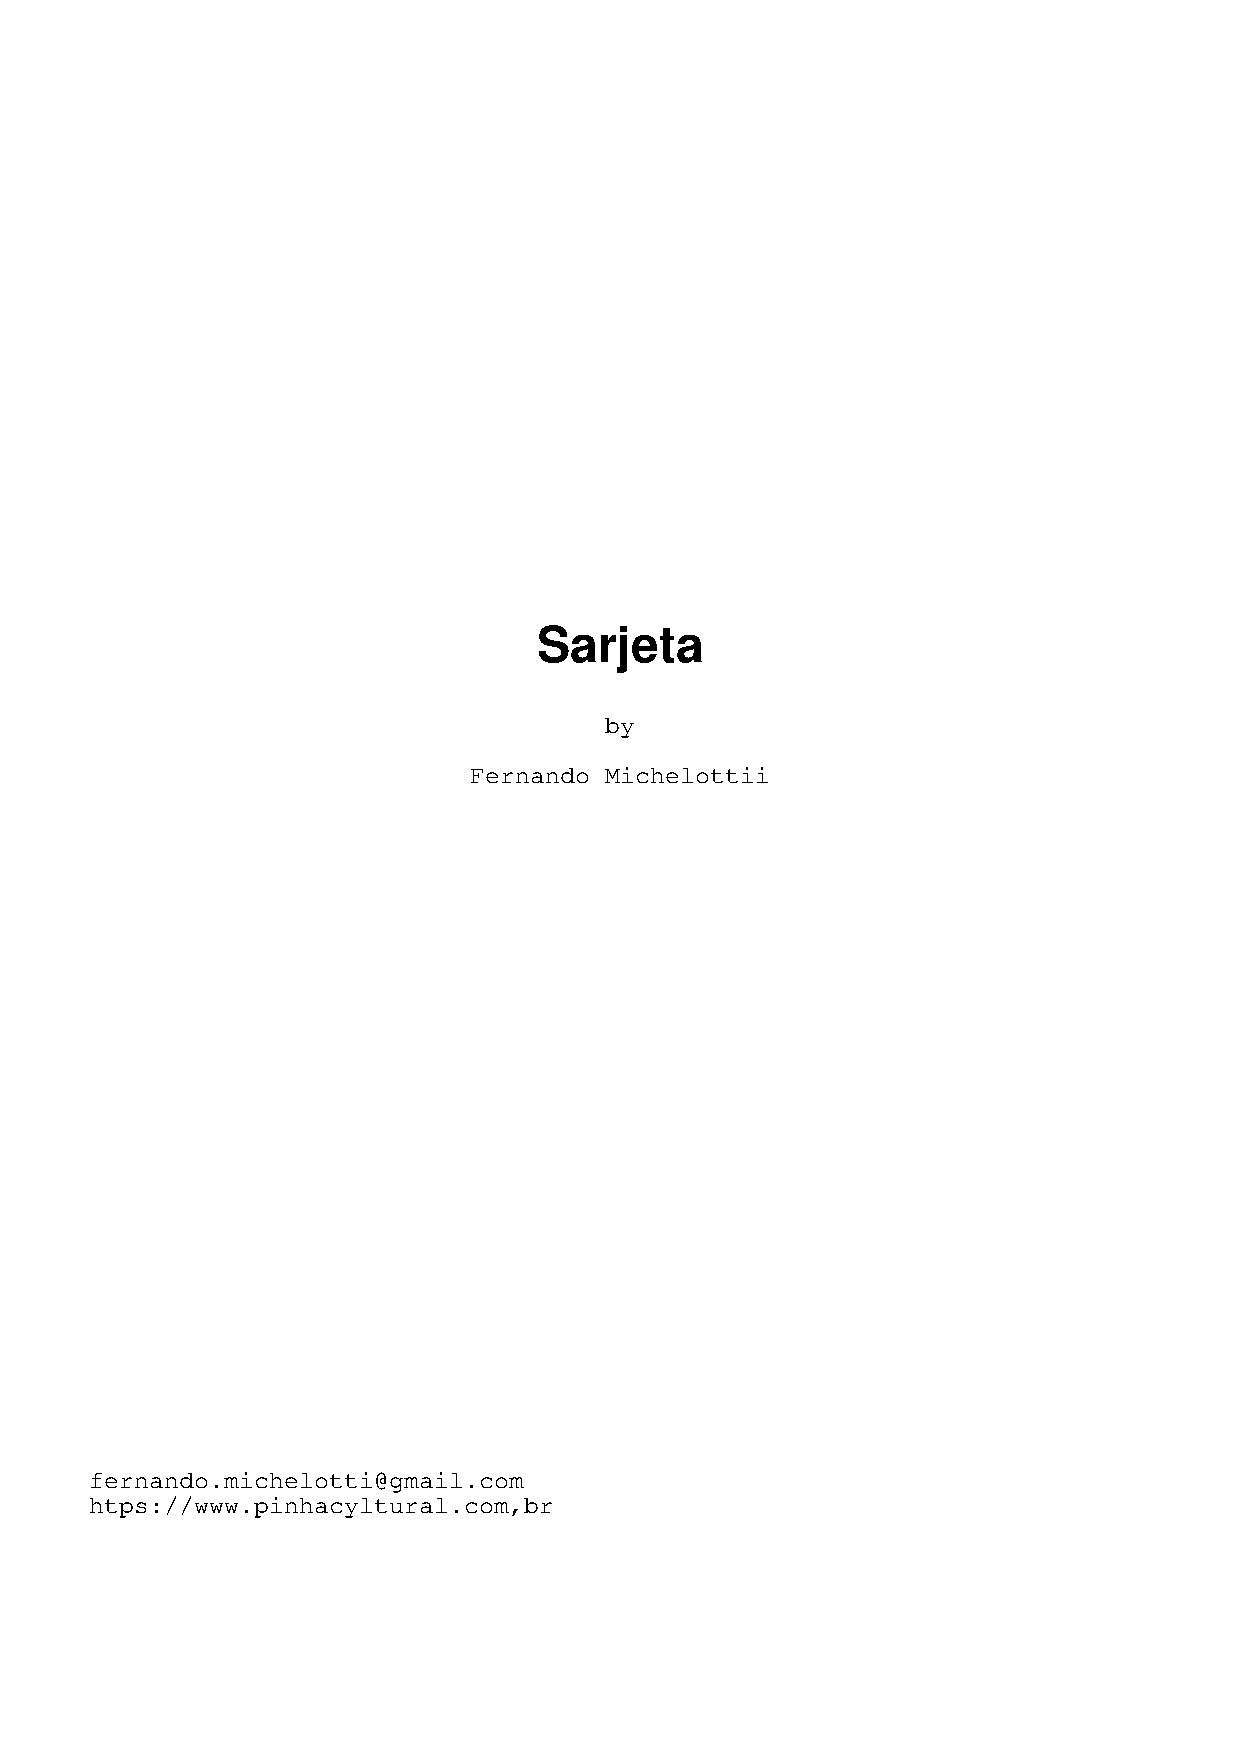
\includepdf[pages=-]{roteiro/roteiro}

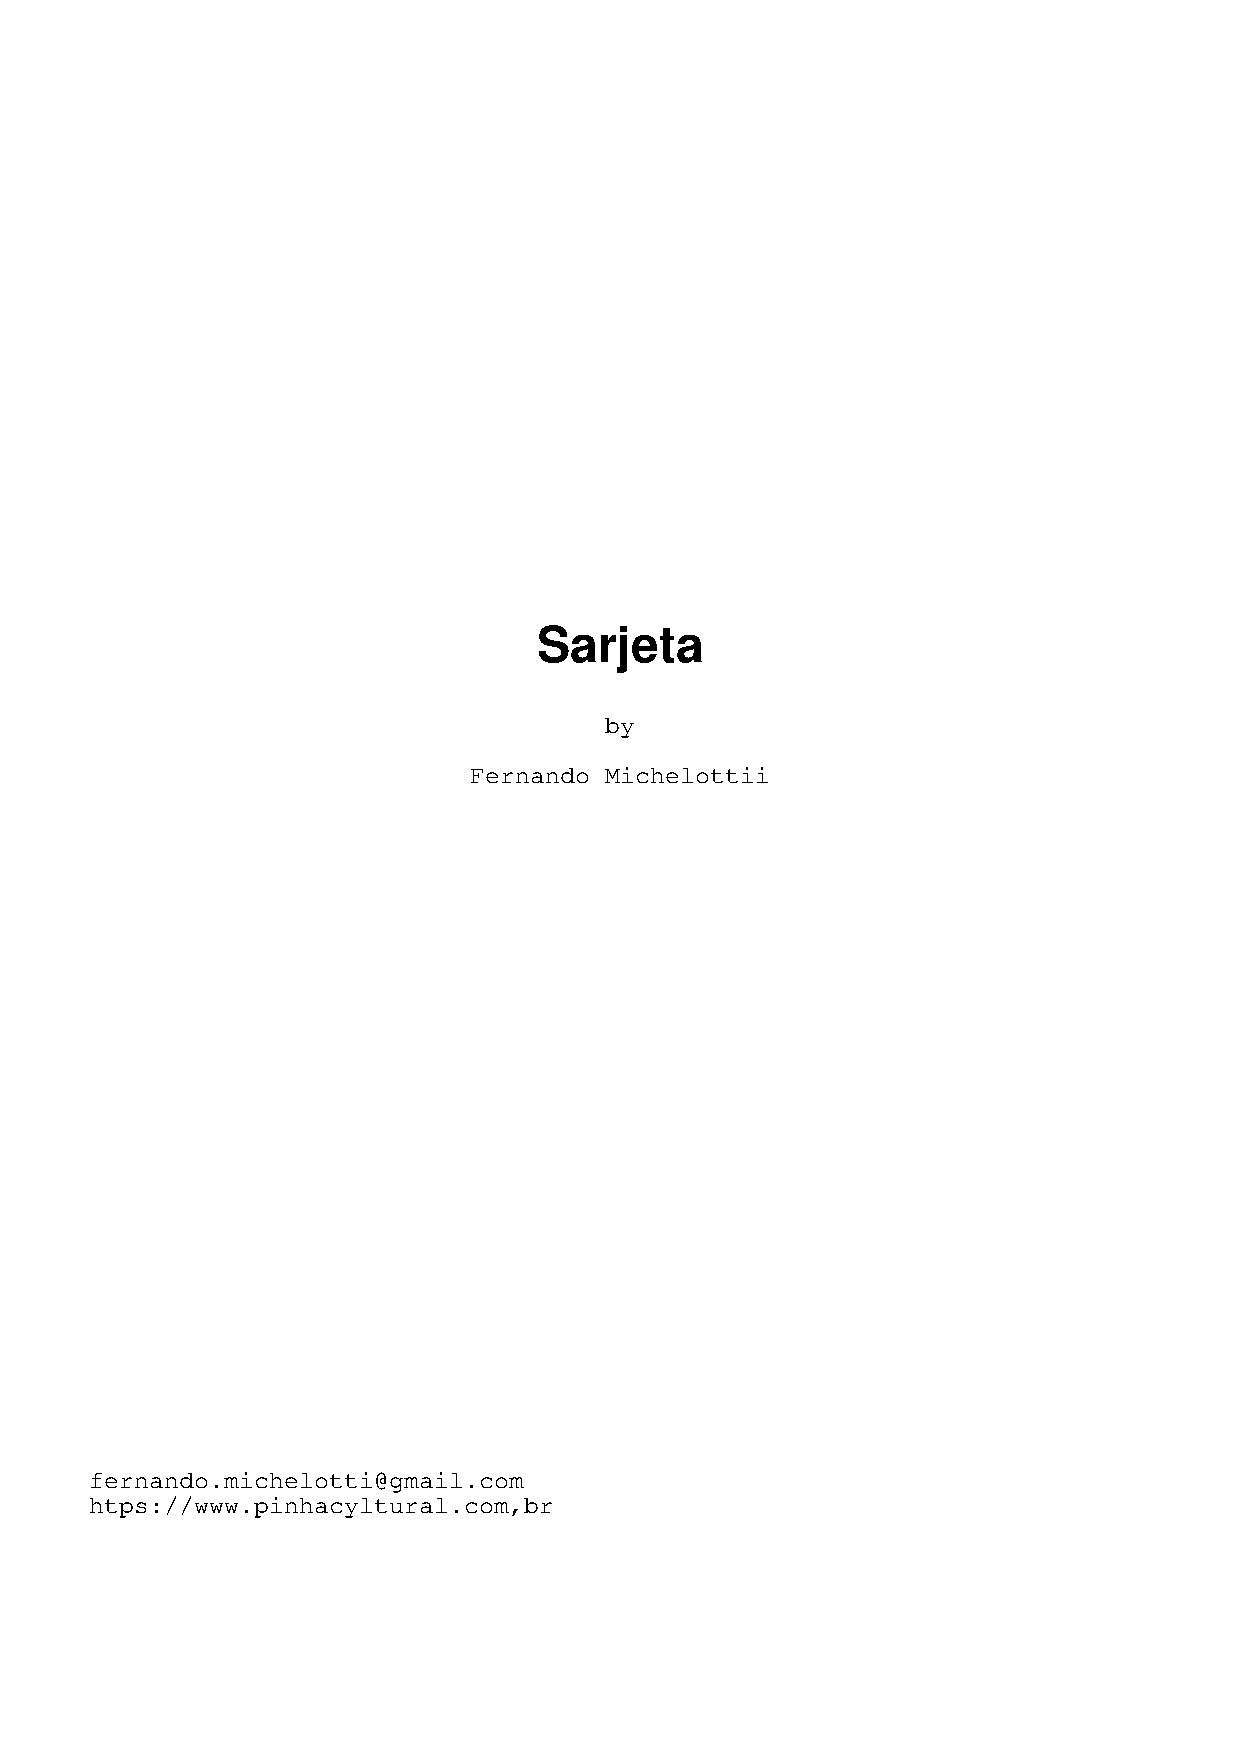
\includepdf[pages=-]{roteiro/roteiro.pdf}

%roteiro/roteiro.pdf

\end{anexosenv}

%---------------------------------------------------------------------
% INDICE REMISSIVO
%---------------------------------------------------------------------

\phantompart

\printindex

\end{document}
